\documentclass{article}
\usepackage[utf8]{inputenc}
\usepackage[margin=0.8in]{geometry}

\title{Binary Indexed Trees}
\author{Justin Zhang}
\date{November 10 2017}

\usepackage{graphicx}

\usepackage{mathtools}
\usepackage{listings}
\usepackage{algorithm}
\usepackage{algorithmicx}
\usepackage[noend]{algpseudocode}

\usepackage{tikz}
\usetikzlibrary{calc,shapes.multipart,chains,arrows,positioning}

\tikzstyle{vertex}=[draw,fill=myseagreen,circle,minimum size=24pt,inner sep=0pt]

\tikzstyle{splitvertex}=[draw,fill=myseagreen,circle split,minimum size=24pt]
\definecolor{mywhite}{RGB}{255,255,255}

\begin{document}

\maketitle

\section{Introduction}
    A Binary Index Tree (BIT), also known as a Fenwick Tree, is used for range sums (usually). Namely, a BIT can do element updates and prefix sums ($a[1]+a[2]+ ... +a[i]$; we one-index BITs for implementation-specific reasons) in $O(\log n)$. This is a tradeoff between a $O(n)$ update/$O(1)$ query prefix-sum solution and the $O(1)$ update/$O(n)$ query naive solution.
    
    BITs are very useful, especially for their simple implementation.
    
\section{BITs}\begin{figure}[h]
\centering
{
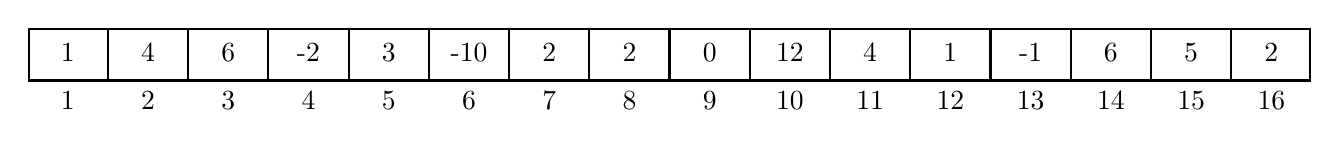
\begin{tikzpicture}[
  thick,
  myrect/.style={
    draw,
    rectangle split,
    rectangle split horizontal,
    rectangle split parts=#1,
    rectangle split part align=left,
    text width=5ex,
    text centered
    },
  mycallout/.style={
    shape=rectangle callout,
    rounded corners,
    fill=mysalmon,
    callout absolute pointer={#1},
    callout pointer width=1cm
  }  
]

\node[myrect=16, rectangle split part fill={mywhite, mywhite, mywhite, mywhite, mywhite, mywhite, mywhite, mywhite, mywhite, mywhite,mywhite, mywhite, mywhite, mywhite, mywhite, mywhite}]
  (array1)
  {
  					\strut 1
  \nodepart{two}	\strut 4
  \nodepart{three}	\strut 6
  \nodepart{four}	\strut -2
  \nodepart{five}	\strut 3
  \nodepart{six}	\strut -10
  \nodepart{seven}	\strut 2
  \nodepart{eight}	\strut 2
  \nodepart{nine}	\strut 0
  \nodepart{ten}	\strut 12
  \nodepart{eleven}	\strut 4
  \nodepart{twelve}	\strut 1
  \nodepart{thirteen}	\strut -1
  \nodepart{fourteen}	\strut 6
  \nodepart{fifteen}	\strut 5
  \nodepart{sixteen}	\strut 2
  };
\foreach \Valor [count=\Valori from 1] in {one ,two ,three ,four ,five ,six ,seven ,eight ,nine ,ten ,eleven ,twelve ,thirteen ,fourteen ,fifteen ,sixteen }
  \node[below] at (array1.\Valor south) {\Valori};

\end{tikzpicture}
}
\caption{A sample array.}
\end{figure}

    BITs rely on the idea that an integer can be decomposed into powers of two. Given an index $i$, we can find these powers of two by writing $i$ in binary. Then, we keep turning off the lowest bit until we reach zero. Say we want to find the prefix sum $a[1]+a[2]+...+a[14]$:
    
    $$ 14 \rightarrow 1110 \rightarrow 1100 \rightarrow 1000 \rightarrow 0 $$
    
    How do we find the prefix sum with this?
    
    Say we just went from $1110 \rightarrow 1100$. We just jumped from index $14 \rightarrow 12$. We can add the elements with indices $13$ and $14$ to a running sum, then recur on $12$:
    
    $$ \texttt{1110 }(14) \xrightarrow[{\texttt{add } a[13]+a[14]}]{} \texttt{1100 }(12) \xrightarrow[{\texttt{add } a[9]+...+a[12]}]{} \texttt{1000 }(8) \xrightarrow[{\texttt{add } a[1]+...+a[8]}]{} 0 $$
    
    Notice that every ``step" (1110, 1100, and 1000), there's a unique range of indices denoted. That is, $\texttt{1110}$ uniquely denotes indices $\texttt{1101}$ and $\texttt{1110}$, or all numbers between the $\texttt{1110}$ and $1+(\texttt{1110} \text{ with the bottom bit removed})$. So we can map every number to a range of indices, and store the sum beforehand; $\texttt{1110}$ stores $a[13]+a[14]$. See the illustration below.

    \begin{figure}
      \center
      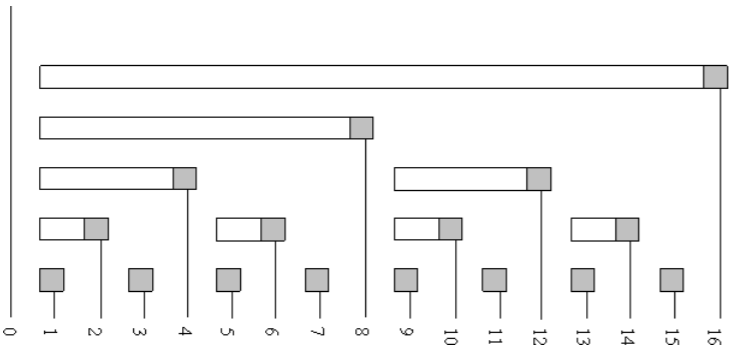
\includegraphics[width=0.525\textwidth]{BIT.PNG}
    \end{figure}
    
    \subsection{Query}
        We discussed query above. But how do we find the lowest bit?
        
        Taking advantage of the two's complement system ($-1 = 1...1111_2, -2 = 1...1110_2$ and so on), we can do this very easily. Say we're using $14 = 1110_2$. $-14 = 0010_2$ (with a bunch of ones in front). If we bitwise AND these two together, we get only the lowest bit set. This holds true in a general sense: let $i = (a1b)_2$, where $a$ and $b$ are parts of the binary number, and the one represents the lowest bit set. Then the negative is as follows: $-i = \textasciitilde(a1b)_2 + 1 = \textasciitilde a0\,\textasciitilde \,b + 1$. But $b$ must consist of only zeros, since it's after the lowest set bit. Thus, we get $-i = (\,\textasciitilde a1b)_2$. Bitwise AND-ing with $i$, we clearly see that only the lowest bit is set.
        
        
        A C++ implementation is shown below.
        \begin{lstlisting}[language=C++]
        int query(int i) {
            int ans = 0;
            for(; i>0; i-=(i & -i))
                ans += a[i];
            return ans;
        }
        \end{lstlisting}
        
        Clearly, to do range queries, we can subtract in the same way we do with regular prefix sums:
        
        \begin{lstlisting}[language=C++]
        int range(int i, int j) {
            return query(j) - (i>1?query(i-1):0);
        }
        \end{lstlisting}
    \subsection{Update}
        To update (add a value $v$) at a given index $i$, we want to add the value to all segments ``above" $i$. Here I mean ``above" in the sense of the diagram above -- all segments that contain $i$.
        
        Let's take $9$. The sequence for segments ``above" 9 is:
        
            $$ \texttt{9 }(1001)\rightarrow \texttt{10 }(1010) \rightarrow \texttt{12 }(1100) \rightarrow{16} (10000). $$
            
        Notice that we're simply adding the lowest bit every time (why?). Then for each index we visit, we add $v$ to the value at this segment. Thus, the implementation is quite similar to query. 
        \begin{lstlisting}[language=C++]
        int update(int i, int v) {
            for(; i<=N; i += (i & -i))
                a[i] += v;
        }
        \end{lstlisting}
        
    Note that for both update and query, we're only going through each bit once. Thus, the complexity is $O(\log n)$.
    
        \subsubsection{Range Updates}
            Range updates are a bit more involved, but can also be done in $O(\log n)$. The idea is to keep two BITs.
            
            Let's say we want to find a given prefix sum to index $i$ (to find the range sum we can still subtract the prefix sums). To do this, we find all ranges that begin before $i$. Then, the answer is:
            
            $$ \sum_{ranges}{max(i, r)*v-(l-1)*v} $$
            
            where $r$ is the right endpoint of a given range, $l$ is the left, and $v$ is the value.
            To calculate this, we can use one BIT to calculate the $i*v$ parts and the other to calculate the $r*v$ and $(l-1)*v$ parts.
            
            Specifically, here's how we'd update:
            \begin{enumerate}
                \item BIT1.update(l, v)
                \item BIT1.update(r+1, -v)
                \item BIT2.update(l, (l-1)*v)
                \item BIT2.update(r+1, -r*v)
            \end{enumerate}
            
            To query $a[1]+...+a[w]$: BIT1.query(w)*w - BIT2.query(w).
            BIT1 handles cases where $w$ falls within a range update; BIT2 handles the endpoints of the range updates.
            
\section{Problems}

\begin{enumerate}
    \item You're given $n$ ($1 \leq n \leq 10^5$) horizontal line segments, each with inclusive endpoints $(x_1, y)$ and $(x_2, y)$ where $-10^9 \leq x_1 \leq x_2 \leq 10^9$. Each line segment has a value $v$ ($-10^9 \leq v \leq 10^9$).

Answer each of $q$ ($1 \leq q \leq 10^5$) queries.
Each query is of the form $x', a, b$, and asks you to sum the values of the $a$-th to the $b$-th (sorted by increasing $y$) line segments at the vertical line $x = x'$.

    \item (Brian Dean, 2012) FJ has set up a cow race with N ($1 \leq N \leq 100,000$) cows running L laps around a circular
track of length C ($1 \leq L, C \leq 25,000$). The cows all start at the same point on the track and run at different
speeds, with the race ending when the fastest cow has run the total distance of $L * C$. FJ notices several
occurrences of one cow overtaking another. Count the total number of crossing events during the entire race.

    \item (Brian Dean, 2011) Farmer John has lined up his N ($1 \leq N \leq 100,000$) cows each with height $H_i$ ($1 \leq H_i \leq
1,000,000,000$) to take a picture of a contiguous subsequence of the cows, such that the median height is at
least a certain threshold X ($1 \leq X \leq 1,000,000,000$). Count the number of possible subsequences.

    \item (SPOJ BRCKTS) Given a bracket expression of length N ($1 \leq N \leq 30,000$), process M operations. There are
two types of operations, a replacement, which changes the i-th bracket into its opposite, and a check, which
determines whether a bracket expression is correct.
\end{enumerate} 
        
\end{document}
